\documentclass{article}
\usepackage[utf8x]{inputenc}
\usepackage{amsmath}
\usepackage{MathUnicode}
\usepackage{upquote,textcomp}
\usepackage[a4paper,bindingoffset=0.2in,left=1in,right=1in,top=1in,bottom=1in,footskip=.25in]{geometry}

\usepackage{changepage}

\usepackage[spanish]{babel}
\usepackage{tabularx}
\usepackage{multirow}
\usepackage{graphicx}
\usepackage{listings}
\usepackage[font=scriptsize]{caption}
\usepackage[font=scriptsize]{subcaption}
\usepackage{caption}
\usepackage[yyyymmdd,hhmmss]{datetime}

\usepackage[colorlinks,urlcolor=blue]{hyperref}

\newcounter{problem}
\newcounter{solution}
\renewcommand{\theenumi}{\alph{enumi}}

\newcommand\Problem{%
  \stepcounter{problem}%
  \textbf{Problema \theproblem.}~%
  \setcounter{solution}{0}%
}

\newcommand\TheSolution{%
  \textbf{Solución:}\\%
}

\newcommand\ASolution{%
  \stepcounter{solution}%
  \textbf{Solución \thesolution:}\\%
}


\setlength{\arrayrulewidth}{1mm}
\setlength{\tabcolsep}{18pt}
\renewcommand{\arraystretch}{1.5}


\author{Pedro Valero Mejía}
\title{Ejercicios de Sistemas Informáticos II}
\parindent 0in
\parskip 1em

\begin{document}

\maketitle
%%%%%%%%%%%%%%%%%%%%%%%%%%%%%%%%%%%%%%%%%%%%%%%%%%%%%%%%%%%%%%%%%%%%%%%%%% PROBLEMA 1
\Problem
Los mensajes llegan a un servidor de descifrado de manera poissoniana con un ritmo medio de llegada de 360 mensajes por minuto. Los tiempos de descifrado son proporcionales a la longitud de los mensajes, los cuales se distribuyen aproximadamente de forma exponencial, con una longitud media de 1500 bytes. La velocidad del servidor de descifrado es de 10Kbyte/s. ¿Cuál es el tiempo medio de espera de respuesta por mensaje? ¿Cuál es el número medio de mensajes en el sistema de descifrado?

\TheSolution

El número de mensajes por unidad de tiempo es la tasa de llegadas, que deberemos escribir en unidades del Sistema Internacional:
\[λ = 360 min^{-1}=6 s^{-1}\]

Por otro lado tenemos que si la longitud del mensaje es una variable aleatoria que sigue una distribución exponencial y el tiempo de procesamiento es proporcional a la longitud, el tiempo de servicio será una variable aleatoria exponencial de media:
\[T_s = \frac{1500 bytes}{10000 bytes/s} = \boxed{0.15s}\]

A partir de aquí podemos calcular la tasa de servicio:
\[μ = \frac{1}{T_s} = 6.66 s^{-1}\]

Se trata de un sistema M/M/1 de modo que podemos calcular el número medio de mensajes en el sistema a partir, únicamente, del factor de utilización según la fórmula:
\[L=\frac{ρ}{1-ρ}=\frac{λ/μ}{1-λ/μ}=\frac{λ/μ}{(μ-λ)/μ}=\frac{λ}{μ-λ}=\boxed{9.09}\]


%%%%%%%%%%%%%%%%%%%%%%%%%%%%%%%%%%%%%%%%%%%%%%%%%%%%%%%%%%%%%%%%%%%%%%%%%% PROBLEMA 2

\Problem
Se tiene un servidor en Internet que recibe un tráfico de Poisson a un ritmo medio P peticiones/s. El tiempo que tarda en atender una petición se encuentra distribuido exponencialmente, siendo capaz de procesar S peticiones/s.

Debido al éxito del servidor, a los quince días de su aparición en Internet su tráfico se ha multiplicado por un factor K. Para resolver el problema, se cambia de ordenador, solicitando uno de potencia K veces superior al actual.

Calcular el nuevo número medio de clientes en el sistema servidor, y el nuevo tiempo de permanencia en el sistema tras la ampliación del servidor en función de los valores anteriores al cambio.

\newpage
\TheSolution

Tras el éxito del servidor pasamos a tener una tasa de llegadas:
\[λ = K \cdot P\]

Al cambiar la potencia del ordenador multiplicándola por $K$ estamos reduciendo el tiempo de servicio según ese mismo factor y multiplicando la tasa de servicio por $K$:
\[μ = S \cdot K\]

Se trata de un sistema M/M/1 donde el número de clientes en el sistema sólo depende del factor de utilización del mismo que, en este caso, no ha cambiado.

Por tanto seguimos teniendo el mismo número medio de clientes en el sistema que antes de producirse los cambios.

Para calcular el nuevo tiempo de permanencia nos apoyamos en el Teorema de Little que nos permite escribir
\[W = \frac{L}{λ}\]
puesto que $L$ no ha cambiado y λ se ha hecho $K$ veces mayor, el tiempo medio de permanencia en el sistema se ha reducido en un factor de $K$.

%%%%%%%%%%%%%%%%%%%%%%%%%%%%%%%%%%%%%%%%%%%%%%%%%%%%%%%%%%%%%%%%%%%%%%%%%% PROBLEMA 3

\Problem
Se desea diseñar un servidor para satisfacer un tráfico de Poisson con un tiempo medio entre peticiones de 10 s. El servicio a proporcionar tiene una duración distribuida exponencialmente con media de 16 s. Calcular:
\begin{enumerate}
\item El número mínimo de servidores para satisfacer el tráfico requerido.
\item Con dicho número de servidores, el tiempo medio de espera en cola por petición.
\item El tiempo medio de espera en cola, en caso de independizar cada servidores, asignándole una cola de espera a cada uno de ellos, y repartiendo el tráfico entre ellos de modo aleatorio para que cada uno reciba la mitad del total.
\end{enumerate}

\TheSolution

\begin{enumerate}
\item

Si nos llega una petición cada 10 segundos, tenemos una tasa de llegadas de
\[λ = 0.1 s^{-1}\]

Dado que el tiempo medio de servicio es de 16s y tenemos $c$ servidores, la tasa de servicio es:
\[μ=\frac{0.0625}{c}\]

Si queremos que el sistema no colapse, necesitamos que el factor de utilización sea menor que 1, es decir:
\[ρ = \frac{λ}{cμ}<1 \implies λ < cμ \implies c>1.6\]
necesitamos $\boxed{2}$ servidores para satisfacer el tráfico requerido
\item

Para este ejercicio nos apoyamos fuertemente en el formulario. Nos encontramos ante un sistema M/M/2 y para calcular el tiempo de espera en cola debemos calcular el número de clientes en el sistema con ayuda de las fórmulas. Una vez obtenido este valor aplicamos el Teorema de Little para calcular el tiempo medio de estancia en el sistema y le restamos el tiempo medio de servicio.

Vamos a ello:

\[ρ = \frac{λ}{2\cdot μ}=0.8\]

\[p_0 = \left[ \sum_{n=0}^{c-1}\frac{(λ/μ)^n}{n!}+\frac{(λ/μ)^c}{c!(1-ρ)}\right]^{-1}=\left[1+1.6+\frac{2.56}{0.4}\right]^{-1}=(9)^{-1}=0.11\]

\[p_2=p_0\frac{c^c}{c!}\left( \frac{λ}{cμ}\right)^n=0.11\cdot 2 \cdot 0.64 = 0.14\]
\[P_q=\frac{p_c}{1-ρ}=0.71\]

Finalmente
\[L=\frac{P_q ρ}{1-ρ}+cρ=4.44\]

Aplicando Little nos queda
\[W = \frac{L}{λ}=44.4\]

Puesto que el tiempo de servicio es de 8s, el tiempo medio de espera en cola asciende a
\[W-T_s=\boxed{36.4s}\]
\item

Este caso es equivalente al ejercicio anterior con $K=0.5$ por lo que tenemos
\[W_n =\frac{W_o}{K}=88.8s\]

lo que implica
\[W-T_s = \boxed{56.8s}\]
\end{enumerate}

%%%%%%%%%%%%%%%%%%%%%%%%%%%%%%%%%%%%%%%%%%%%%%%%%%%%%%%%%%%%%%%%%%%%%%%%%% PROBLEMA 4

\Problem
Se quiere diseñar un servidor de emisión de certificados en Internet para que sea capaz de atender una media de 10 peticiones por segundo con un tiempo medio de respuesta de 0.1s. Sabiendo que el programa de generación del certificado es siempre el mismo, independientemente del cliente, y requiere la ejecución de 10.000 instrucciones de código máquina, calcular la potencia de ordenador (en MIPS) necesaria para su ejecución,
suponiendo despreciable cualquier otra carga en el mismo.

\TheSolution

Queremos ejecutar 10.000 instrucciones de código en 0.1s deberemos tener una potencia de \boxed{0.1 MIPS}


%%%%%%%%%%%%%%%%%%%%%%%%%%%%%%%%%%%%%%%%%%%%%%%%%%%%%%%%%%%%%%%%%%%%%%%%%% PROBLEMA 5

\Problem
Una fracción p del tráfico de salida procedente de un servidor con tiempo de servicio distribuido exponencialmente con media Ts se realimenta a su entrada. El tráfico nuevo llega al servidor con un ritmo medio R. Calcular el factor de utilización del servidor y el tiempo medio de estancia en el
sistema.

\TheSolution

Empezamos calculando la tasa de llegadas:
\[λ = R + pλ \implies λ = \frac{R}{1-p}\]

La taasa de servicio es
\[μ= \frac{1}{T_s}\]

Así el factor de utilización sería
\[ρ=\frac{λ}{μ}=\boxed{\frac{R \cdot T_s}{1-p}}\]

Sabiendo que es un sistema M/M/1 podemos calcular el número medio de clientes en el sistema como:
\[L = \frac{ρ}{1-ρ}=\frac{R\cdot T_s}{1-p-R\cdot T_s}\]

Aplicando ahora el Teorema de Little podemos calcular el tiempo medio de estancia en el servidor como:
\[W = \frac{L}{λ}=\boxed{\frac{T_s}{(1-p-R\cdot T_s)(1-p)}}\]

%%%%%%%%%%%%%%%%%%%%%%%%%%%%%%%%%%%%%%%%%%%%%%%%%%%%%%%%%%%%%%%%%%%%%%%%%% PROBLEMA 6

\Problem
En una determinada red de área local se dispone de un servidor de comunicaciones, que actúa como encaminador de mensajes de aplicación entre la dicha red y una red remota, a la que se encuentra conectado a través de una línea dedicada de velocidad $2\cdot 10^6$ bps.

A la red de área local hay conectados un número muy grande de terminales clientes, que envían mensajes cuyo tamaño se encuentra distribuido exponencialmente con un valor medio de 1 KByte.

Se puede considerar que los mensajes llegan al servidor siguiendo un ritmo de Poisson. Se pide:
\begin{enumerate}
\item Si el servidor de comunicaciones recibe un promedio de 180 peticiones/s, calcular tiempo medio que transcurre desde que un mensaje es recibido en el servidor hasta que llega al punto destino.
\item Calcular el número máximo de peticiones por segundo que se estarán procesando si se sabe que el tamaño medio de memoria que ocupa la cola de mensajes en espera de ser procesados es de 10 KBytes.
\end{enumerate}

\TheSolution

En este ejercicio el tiempo de procesamiento de mensaje por parte del servidor es el tiempo que tarda dicho servidor en enviar el mensaje a través del enlace descrito.

\begin{enumerate}
\item
Tenemos una tasa de peticiones
\[λ = 180 s^{-1}\]

Sabiendo el tamaño medio de los mensajes y la capacidad de transmisión de la línea dedicada, podemos calcular el tiempo de servicio
\[T_s = \text{tamaño}/\text{velocidad} = 0.0041s\]

lo que nos da una tasa de servicio de
\[μ=\frac{1}{T_s}=244.14 s^{-1}\]

A partir de aquí podemos calcular el factor de utilización del sistema
\[ρ = \frac{λ}{μ}=0.74\]

y, puesto que estamos ante un sistema M/M/1 podemos calcular el número medio de clientes en el sistema como
\[L = \frac{ρ}{1-ρ}=2.85\]
y a partir del Teorema de Little calculamos el tiempo medio de estancia en el sistema, que es el dato pedido
\[W= \frac{L}{λ}= \boxed{0.016s}\]

\item

Ahora nos encontraríamos ante un sistema M/M/1/K siendo $K$ el número máximo de clientes en el sistema que se calcula como el número máximo de clientes en cola +1 (el que se está procesando).

Puesto que conocemos el tamaño de la cola y el tamaño de los mensajes, podemos calcular $K=10$ mensajes. Es decir, tenemos un sistema M/M/1/10 y nos piden calcular $L$, el número máximo de clientes en el sistema.

Los valores de λ y μ calculados en el apartado anterior siguen siendo válidos, pues no han cambiado las condiciones de llegada y procesamiento de mensajes.

Procedemos pues a calcular $L$:
\[L = \frac{λ/μ}{1-λ/μ}\frac{1-(K+1)(λ/μ)^K+K(λ/μ)^{K+1}}{1-(λ/μ)^{K+1}}=\frac{λ/μ}{1-λ/μ}\frac{1-(3)(λ/μ)^2+2(λ/μ)^{3}}{1-(λ/μ)^{3}}=\]
\[=\frac{0.74}{0.26}\frac{0.17}{0.6}=\boxed{0.81}\]

\end{enumerate}
%%%%%%%%%%%%%%%%%%%%%%%%%%%%%%%%%%%%%%%%%%%%%%%%%%%%%%%%%%%%%%%%%%%%%%%%%% PROBLEMA 7

\Problem
Deseamos instalar un servidor de envío de mensajes ("busca") a una serie de abonados. El número de abonados, que suponemos muy grande, envía mensajes a nuestro servidor, desde donde se envían a su destino mediante un sistema de transmisión por radio. Los mensajes llegan según un proceso de Poisson con una tasa de llegadas L. El tiempo de servicio (total del proceso y envío del mensaje) se puede considerar distribuido exponencialmente con valor medio S. El esquema de bloques del servicio es el siguiente:

\begin{center}
  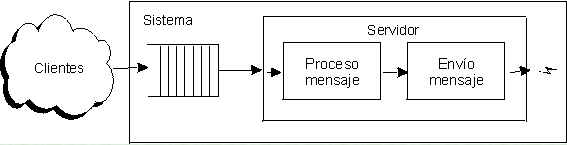
\includegraphics[keepaspectratio=true,width=\linewidth]{ej7.png}
  \captionof{figure}{Consola de Glassfish}
\end{center}


\begin{enumerate}
\item Calcular el tiempo medio que transcurre desde que un mensaje llega al sistema hasta que es servido a su destino.
\item La tarifa del servicio es de P Euros por mensaje transmitido, pero se proporciona un descuento de D Euros por cada segundo que el mensaje tarde en llegar a su destino. Calcular los ingresos medios esperados por mensaje transmitido.
\item Calcular a partir de qué tasa de peticiones el tiempo de espera será tal que el mensaje se deba transmitir gratuitamente (se supone que nunca se aplica un descuento mayor que el coste de transmisión del mensaje).

\end{enumerate}

\newpage
\TheSolution

\begin{enumerate}
\item
Tenemos las tasas de llegadas y servicio
\[λ=L \ \ \ μ=\frac{1}{S}\]

A partir de estos datos calculamos el factor de utilización
\[ρ = \frac{λ}{μ}=L\cdot S\]

Puesto que nos encontramos ante un sistema M/M/1 podemos calcular el número de clientes en el sistema a partir del factor de utilización:
\[L_c=\frac{ρ}{1-ρ}=\frac{L}{S-L}\]

Por último calculamos el tiempo medio de estancia en el sistema a partir del teorema de Little:
\[W = \frac{L_c}{λ}=\frac{L\cdot S}{S-L_c}\]

\item

Los ingresos medios serán el precio por mensaje por el número medio de mensajes que se manipulan menos el dinero que se devuelve por segundo de retraso multiplicado por el retraso habitual de procesamiento de los mensajes.

Nos queda la fórmula
\[\text{Ingresos} = P \cdot L_c - D \cdot W\]

\item

Basta con igualar los ingresos a 0:
\[P\cdot L_c = D \cdot W \iff P \cdot L_c = \frac{L\cdot S}{S-L_c} \]
Ahora simplemente despejamos $L_c$ y a partir de ahí despejamos ρ que usaremos para calcular λ.

\end{enumerate}

%%%%%%%%%%%%%%%%%%%%%%%%%%%%%%%%%%%%%%%%%%%%%%%%%%%%%%%%%%%%%%%%%%%%%%%%%% PROBLEMA 8

\Problem
Una red de una entidad financiera consta de una serie de terminales remotos, en número que podemos considerar muy grande, conectados mediante líneas telefónicas alquiladas full duplex a un multiplexor de terminales. Dicho multiplexor entrega los mensajes recibidos a un servidor, que ejecuta los programas transaccionales necesarios para atender al mensaje recibido, y devuelve los resultados al cliente a través del mismo multiplexor. El esquema de bloques del servicio es el siguiente:

\begin{center}
  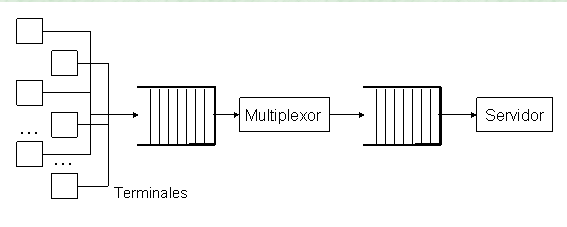
\includegraphics[keepaspectratio=true,width=\linewidth]{ej8.png}
  \captionof{figure}{Consola de Glassfish}
\end{center}

Los mensajes de las oficinas llegan al multiplexor según un proceso de Poisson con una tasa de llegadas total de 3 s -1 (es decir, incluyendo las peticiones de todos los servidores) y su longitud media es de 1 Kbyte. El tiempo de servicio del multiplexor por mensaje (total del proceso y envío del mensaje) se puede considerar distribuido exponencialmente con valor medio 250 ms.

\begin{enumerate}
\item Calcular la ocupación media en memoria de la cola de mensajes en espera de servicio del multiplexor
\item Calcular la tasa de llegadas al servidor.
\item Los mensajes que llegan al servidor son de tres tipos básicos. El tiempo de proceso en el servidor depende del tipo de mensaje recibido, de acuerdo a la siguiente tabla:

\begin{center}
\begin{tabular}{| c | c | c |}
\hline
  \textbf{Identificador mensaje} &  \textbf{Probabilidad} & \textbf{Tiempo de proceso}\\
\hline
0 & 0.5 & 0.1 \\
1 & 0.3 & 0.2 \\
2 & 0.2 & 0.4 \\
\hline
\end{tabular}
\end{center}

Estos tiempos incluyen lo que tarda el mensaje de respuesta en llegar al terminal remoto. Esta transmisión del mensaje de respuesta se supone que no afecta al tiempo de proceso del multiplexor ni a la comunicación por la línea que lo une con el terminal.

Calcular el tiempo medio de estancia en el servidor de las solicitudes.


\end{enumerate}

\TheSolution

\begin{enumerate}

\item

Tenemos una tasa de llegadas $λ=3$ y un tiempo de servicio por parte del multiplexor de 250ms lo que nos da una tasa de servicio $μ=4$.

Analizando por separado el multiplexor, tenemos un sistema M/M/1 de modo que calculamos ρ y lo usamos para calcular el número medio de clientes $L$.

\[π=\frac{λ}{μ}=0.75\]
\[L=\frac{ρ}{1-ρ}=3\]

\item

La tasa de llegadas al servidor es exactamente la misma que la tasa de llegadas al multiplexor. Cada mensaje que llega a este último es enviado al servidor

\item

El tiempo de servicio en el servidor se puede calcular como una suma ponderada de los tiempos de servicio de cada tipo de mensaje.
\[T_s = 0.5\cdot 0.1+0.3\cdot 0.2+0.2\cdot 0.4=0.19 \implies μ = \frac{1}{T_s}=5.26\]

Volvemos a tener un sistema M/M/1. Calculamos ρ, a partir de ahí $L$ y por último empleamos el Teorema de Little para calcular el tiempo medio de estancia en el sistema.

\[ρ = \frac{λ}{μ}=0.57 \implies L=\frac{ρ}{1-ρ}=1.33 \implies W = \frac{L}{λ}=0.44 s\]
\end{enumerate}

\newpage
%%%%%%%%%%%%%%%%%%%%%%%%%%%%%%%%%%%%%%%%%%%%%%%%%%%%%%%%%%%%%%%%%%%%%%%%%% PROBLEMA 9

\Problem
El servidor de fecha y hora de una red resuelve cada petición en un tiempo que se puede suponer distribuido exponencialmente con media 100 ms. La red se compone de un número muy grande de clientes que realizan peticiones, cuya llegada al servidor se considera que sigue un proceso de Poisson.
\begin{enumerate}
\item Calcular el número máximo de peticiones por segundo que se podrán satisfacer para obtener un tiempo medio de respuesta del servidor menor o igual que 1 s.
\item Calcular el tiempo medio de servicio necesario para poder satisfacer el doble de peticiones reduciendo el tiempo de respuesta a la mitad.

\end{enumerate}

\TheSolution

\begin{enumerate}
\item Nos piden calcular el número máximo de peticiones por segundo que se pueden satisfacer, es decir, tenemos que calcular λ.

Sabemos que el tiempo medio de servicio es de 100 ms, por lo que tendremos que
\[μ = \frac{1}{T_s}=\frac{1}{100 ms} = \frac{1}{0.1s}=10s^{-1}\]

El tiempo de servicio es el tiempo medio de estancia en el sistem y queremos que sea menor que 1, por lo que:
\[W=\frac{L}{λ}=\frac{\rho}{λ(1-\rho)}=\frac{1}{μ-λ} < 1 \implies μ > λ +1\]
por lo que el sistema no podrá atender más de 9 peticiones por segundo.

\item Ahora queremos que λ=18 manteniendo el tiempo medio de respuesta de 1 s. Sustituyendo en la ecuación anterior tenemos:

\[W < \frac{1}{2} \implies μ > λ +2 \implies μ > 20 \implies T_s < \frac{1}{20} = 50 ms\]
\end{enumerate}

%%%%%%%%%%%%%%%%%%%%%%%%%%%%%%%%%%%%%%%%%%%%%%%%%%%%%%%%%%%%%%%%%%%%%%%%%% PROBLEMA 10

\Problem
Un servidor web de aplicaciones se compone de los siguientes elementos

\begin{center}
  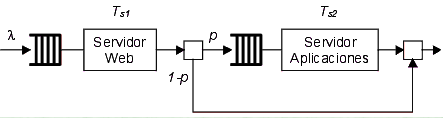
\includegraphics[keepaspectratio=true,width=\linewidth]{ej10.png}
  \captionof{figure}{Consola de Glassfish}
\end{center}

La llegada de solicitudes al sistema se puede considerar como un proceso de Poisson, con una tasa de llegadas de 6 peticiones por segundo. Existe un número muy grande de clientes, de modo que el número de peticiones pendientes de servicio no afecta al ritmo de llegada de nuevas peticiones.

El servidor Web atiende las peticiones de páginas estáticas e imágenes, empleando para ello un tiempo que se puede considerar distribuido exponencialmente con un valor medio de 50 ms. Se considera que el servidor procesa las peticiones de modo iterativo, es decir, de una en una.

Un 10\% de las peticiones procesadas por el servidor web requieren que, adicionalmente al proceso realizado por dicho servidor, se ejecute un programa externo. Esta ejecución se realiza en un servidor de aplicaciones, cuyo tiempo de servicio también se puede considerar distribuido exponencialmente con un valor medio de 1 s. También en este caso se considera que el servidor procesa las peticiones de modo iterativo.

\begin{enumerate}
\item Calcular el tiempo medio de estancia en el sistema de las peticiones que atiende únicamente el servidor Web, justificando el modelo de cálculo elegido.

\item Calcular el tiempo medio de estancia en el sistema de las peticiones que necesitan ser atendidas por ambos servidores, justificando el modelo de cálculo elegido.

\item Calcular el tiempo medio de estancia en el sistema total.

\item Realizando medidas sobre el sistema en producción se descubre que el tiempo de servicio del servidor web no sigue una distribución exponencial, sino una distribución cuyo coeficiente cuadrático de variación es igual a 5. Justificar la validez o invalidez del modelo empleado en los apartados anteriores, indicando las alternativas si no se considera válido.
\end{enumerate}

\TheSolution

\begin{enumerate}
\item
Para esta parte podemos suponer que el sistema se acaba al salir del servidor de modo que nos encontramos ante un sistema M/M/1 bastante sencillo. Vamos a calcular el tiempo medio de estancia en ese sitema reducido como hacemos siempre.

\[λ = 6, T_s = 50 ms \implies μ=\frac{1}{T_s}=20 \implies ρ = \frac{λ}{μ}=0.3\]

\[L=\frac{ρ}{1-ρ}=0.43 \implies W = \frac{L}{λ}=0.07s\]

\item

Puesto que no tenemos retroalimentación, la tasa de llegadas a este segundo sistema sería del 10\% de la tasa de llegadas al Servidor Web. Calculamos este nuevo λ y repetimos los cálculos del apartado anterior.

\[λ = 0.1\cdot 6 = 0.6, T_s = 1 s \implies μ=\frac{1}{T_s}=1 \implies ρ = \frac{λ}{μ}=0.6\]

\[L=\frac{ρ}{1-ρ}=1.5 \implies W = \frac{L}{λ}=15s\]

\item

\[W = W_{s_1}+p\cdot W_{s_2} = 1.57s\]

\item

El modelo empleado no será válido ya que para serlo el coeficiente cuadrátido de variación debería ser muy próximo a 1, cosa que no se cumple.

A fin de ajustar las estimaciones deberíamos repetir los cálculos considerando una distribución de tipo hiperexponencial

\end{enumerate}


%%%%%%%%%%%%%%%%%%%%%%%%%%%%%%%%%%%%%%%%%%%%%%%%%%%%%%%%%%%%%%%%%%%%%%%%%% PROBLEMA 11

\Problem Un middleware orientado a colas de mensajes (MOM) recibe mensajes en una cola local de todos los ordenadores que componen la red de modo aleatorio. La llegada de mensajes al MOM se puede considerar como un proceso de Poisson, con una tasa de llegadas de 10 peticiones por segundo. Existe un número muy grande de clientes, de modo que el número de peticiones pendientes de servicio no afecta al ritmo de llegada de nuevas peticiones. La longitud de los mensajes que se recibe es de 25Kbytes. El tamaño disponible para almacenar mensajes en la cola se supone ilimitado. Los mensajes recibidos en esta cola son procesados por dos servidores. El tiempo de servicio en cualquiera de ellos se puede considerar distribuido exponencialmente con un valor medio de 50 ms. Tan pronto como uno de los servidores esté libre, tomará el primer mensaje de la cola y lo procesará sin interrupciones.
\begin{enumerate}
\item Calcular el tamaño medio, en Kbytes, que tendrá la cola de mensajes en el MOM.
\item Calcular el tiempo medio de estancia en el sistema de las peticiones de los clientes.
\item Calcular cuál es la probabilidad de que el tamaño de la cola de mensajes sea mayor de 100 Kbytes.
\end{enumerate}

\TheSolution

Los datos que podemos extraer del enunciado son:
\[\left\{
\begin{array}{l}
λ = 10 \\
\text{Longitud de mensaje } 25Kb \\
\text{Colas infinitas} \\
\text{2 servidores con tiempo de servicio exponencial} \\
T_s = 50ms
\end{array}
\right.\]

Antes de hacer ningún cálculo, reconocemos que se trata de un modelo M/M/2
\begin{enumerate}
\item
Para calcular el tamaño medio de la cola de mensajes basta con calcular el número medio de mensajes en la cola y multiplicarlo por el tamaño de cada mensaje.

Por el teorema de Little tenemos

\[L_q = λ W_q\]

Pero sabemos que el tiempo de estancia en el sistema es la suma del tiempo de servicio más el tiempo de espera en cola, de modo que
\[L_q = λ w_q = λ (W-T_s)\]

y aplicando nuevamente el teorema de Little para calcula W tenemos:
\[L_q = λ\left(\frac{L}{λ}-\frac{1}{μ}\right)=L-cρ\]

Empezamos calculando el factor de utilización del sistema:
\[ρ = \frac{λ}{2μ}=\frac{λT_s}{2}=10\cdot 25ms = 0.25\]

Calculemos ahora el número medio de unidades en el sistema:
\[L=\frac{P_qρ}{1-ρ}+cρ\]
pero antes necesitamos conocer $P_q$:

\[P_q = \frac{p_c}{1-ρ}\]
y para ello necesitamos $p_c$ siendo $c=2$.

Para calcular $p_2$ tenemos que emplear la fórmula:
\[p_2=p_0\frac{c^c}{c!} \left(\frac{λ}{cμ}\right)^n\]

para lo que necesitamos conocer $p_0$.

\[p_0 = \left(1+0.5+\frac{0.5^2}{2\cdot 0.75}\footnote{Puesto que ρ < 1}\right)^{-1} = \frac{1}{1.64}=0.6\]

Una vez tenemos esto podemos calcular $p_2$.
\[p_2=p_0\frac{c^c}{c!} \left(\frac{λ}{cμ}\right)^n=0.6\cdot \frac{4}{2}\cdot (0.25)^2 = 0.075\]

Con este valor procedemos a calcular $P_q$:
\[P_q = \frac{p_c}{1-ρ} = \frac{0.075}{0.75}=0.1\]

Y ya estamos en condiciones de calcular $L$:
\[L=\frac{P_qρ}{1-ρ}+cρ = \frac{0.1\cdot 0.25}{0.75}+2\cdot 0.25 = 0.53\]

Ahora calculamos $L_q$
\[L_q = L -cρ = 0.53 - 2 \cdot 0.25 = 0.03\]

Y por último multiplicamos por el tamaño de cada mensaje:
\[\text{ Tamaño medio = } 0.03\cdot 25 Kb = 0.75KB\]
\item

El tiempo medio de estancia en el sistema puede calcularse, a partir del Teorema de Little, como:
\[W = \frac{L}{λ} = \frac{0.53}{10} = 0.053\]


\item La probabilidad de que el tamaño de la cola de mensajes sea mayor de 100 Kb equivale a la probabilidad de tener más de 4 mensajes en la cola que, a su vez, equivale a la probabilidad de que haya más de 6 clientes en el sistema.

Vamos a calcular esta probabilidad:
\[P\{N(t) \geq 7\} = \sum_{n=6}^{\infty} p_0\cdot \frac{c^c}{c!} \cdot ρ^n=p_0\cdot \frac{c^c}{c!} \cdot ρ^6 \sum_{n=6}^{\infty}ρ^{n-6} =p_0\cdot \frac{c^c}{c!} \cdot ρ^7 \frac{1}{1-ρ} = \frac{0.6\cdot 2 \cdot 6.10 \cdot 10^{-5} }{0.75}=9.76 \cdot 10^{-5}\]
\end{enumerate}

%%%%%%%%%%%%%%%%%%%%%%%%%%%%%%%%%%%%%%%%%%%%%%%%%%%%%%%%%%%%%%%%%%%%%%%%%% PROBLEMA 12

\Problem
Para dar servicio de consultas a base de datos en una red se dispone de dos ordenadores. El primero, que llamaremos A, tiene un tiempo medio de servicio de 100 ms., pero por construcción sólo admite 5 peticiones en espera de servicio. El segundo, que llamaremos B, tiene un tiempo medio de servicio de 500 ms., pero admite un número ilimitado de peticiones en cola de espera. Los tiempos de servicio de ambos servidores se pueden considerar distribuidos exponencialmente. La arquitectura que se decide para dar el servicio coloca los dos servidores en paralelo. Las peticiones serán procesadas por el servidor A, excepto en el caso de que éste se encuentre al máximo de su capacidad (5 peticiones en cola mas una en servicio), en cuyo caso la petición será pasada al servidor B. La llegada de consultas al sistema se puede considerar como un proceso de Poisson, con una tasa de llegadas de 9 peticiones por segundo. Existe un número muy grande de clientes, de modo que el número de peticiones pendientes de servicio no afecta al ritmo de llegada de nuevas peticiones.

\begin{itemize}
\item Calcular el tiempo medio de estancia en el sistema de las peticiones que son procesadas por el servidor A.
\item Calcular el tiempo medio de estancia en el sistema total compuesto por los servidores A y B.
\end{itemize}

\TheSolution

%%%%%%%%%%%%%%%%%%%%%%%%%%%%%%%%%%%%%%%%%%%%%%%%%%%%%%%%%%%%%%%%%%%%%%%%%% PROBLEMA 13
\Problem En una instalación se tiene un problema con el tiempo de respuesta de un servidor de RPCs. El ordenador en el que reside dicho servicio tiene 2 CPUs dedicadas exclusivamente a procesar las peticiones, de modo que cualquiera de ellas puede atender cualquier petición en cualquier estado, y un sistema de disco único. El tráfico de llegada al servidor se puede suponer de Poisson, con un valor medio de R peticiones por segundo.

El proceso que se efectúa en el servidor necesita realizar un número variable de accesos a disco. Se ha estimado que cada petición emplea un tiempo de proceso en alguna de las CPUs que se encuentra distribuido exponencialmente con un valor medio T1. Transcurrido este periodo, la petición necesita acceder a disco con una probabilidad p, o finaliza en caso contrario.

El acceso al único disco del sistema emplea un tiempo distribuido exponencialmente, con un valor medio de T2.
Una vez realizado el acceso a disco, la petición volverá siempre a la cola de entrada en espera nuevamente de que alguna de las CPUs esté libre para continuar el proceso.

El tamaño de las colas de espera en cualquier parte del sistema se puede considerar infinito.

Datos numéricos: R = 2$s^{-1}$; p = 0.8; T1 = 20 ms.; T2 = 100 ms.
\begin{enumerate}
\item Dibujar el diagrama de bloques del sistema, indicando en él los puntos de encolamiento, tasas de peticiones recibidas en cada punto y tiempos de servicio de cada uno de los elementos que lo componen.
\item Calcular el número medio de unidades en cola en el sistema total.
\item Calcular el tiempo medio de estancia en el sistema de una petición.
\item A partir de los resultados obtenidos, identificar los ``cuellos de botella'' del sistema, y realizar sugerencias sobre las modificaciones que sería necesario introducir en el mismo para reducir el tiempo medio de estancia en él.
\end{enumerate}
\TheSolution

\begin{enumerate}
\item Se trata de una red de colas M/M/1

\item
El número medio de unidades en cola será la suma del número medio de unidades en cada una de las colas.

Las tasas de llegadas de cada cola son:
\[λ_1 = R + p \cdot λ_1 \implies λ_1 - p\cdot λ_1 = R \implies λ_1 = \frac{R}{1-p} = 10 s^{-1}\]
\[λ_2 = p\cdot R + p \cdot λ_2 \implies λ_2 - p\cdot λ_2 = p \cdot R \implies λ_2 = \frac{p\cdot R}{1-p} = p\cdot 10 s^{-1} = 8 s^{-1}\]

Conocemos ya los tiempos de servicio de cada ``subsistema'' de modo que podemos calcular las tasas de servicio:
\[μ_1 = \frac{1}{T_1/2}=100s^{-1}\]
\[μ_2 = \frac{1}{T_2}=10s^{-1}\]

Conocidos estos valores podemos calcular el factor de utilización de cada ``subsistema'' y con él el número medio de clientes en cada ``subsistema'':
\[ρ_1 = \frac{λ_1}{μ_1}=0.1 \implies L_1=\frac{ρ_1}{1-ρ_1} = 0.11\]
\[ρ_2 = \frac{λ_2}{μ_2}=0.8 \implies L_2=\frac{ρ_2}{1-ρ_2} = 4\]

Aplicando el teorema de Little podemos calcular el tiempo de estancia en cada ``subsistema'':
\[W_1 = \frac{L_1}{λ_1} = 0.011 s\]
\[W_2 = \frac{L_2}{λ_2} = 0.5 s\]

Sabiendo que el tiempo medio de estancia en el ``subsistema'' es la suma del tiempo medio de espera en cola más el tiempo medio de servicio, podemos calcular el tiempo medio de espera en cola de cada ``subsistema'' es que:
\[TC_1 = W_1-T1/2 = 1 ms = 0.001 s\]
\[TC_2 = W_2-T2 = 400 ms = 0.4s\]

Aplicando nuevamente el teorema de little podemos calcular el número medio de clientes en cada cola:
\[Lq_1 = λ_1TC_1 = 0.01\]
\[Lq_2 = λ_2TC_2 = 3.2\]

El número medio de clientes en cola en el sistema total será la suma del número medio de clientes en cada una de las colas, es decir, tenemos que
\[Lq = Lq_1+Lq_2 = 3.21 \text{clientes}\]

\item

El tiempo medio de estancia en el sistema de una petición se calcula de la siguiente forma:
\[W = \frac{\sum L_i}{\sum α_i}=2.06s\]

También podríamos calcularlo como:
\[W = W_1+pW_2+pW \implies W = \frac{W_1+pW_2}{1-p}=2.06s\]

Estamos teniendo en cuenta el hecho de que no todas las peticiones pasan por ambos ``subsistemas'' al multiplicar por $p$.

Por otro lado estamos considerando la recursividad a la hora de calcular la tasa de llegadas a cada uno de los ``subsistemas'', dato en que nos hemos basado para calcular los tiempos medios de estancia.

\item

A partir de estos datos podemos observar que el cuello de botella en el sistema es el acceso al disco que, por ser disco único y tener tiempo de acceso 5 veces mayor que el tiempo de procesamiento en cada una de las 2 CPUs, lleva 10 veces más tiempo que el procesamiendo de la petición.

Habría que disminuir este tiempo mediante una sustitución del disco por uno más rápido, permitiendo múltiples accesos simultáenos al disco o aumentando el número de discos.

\end{enumerate}

%%%%%%%%%%%%%%%%%%%%%%%%%%%%%%%%%%%%%%%%%%%%%%%%%%%%%%%%%%%%%%%%%%%%%%%%%% PROBLEMA 14

\Problem
Basándose en los conceptos de teoría de colas expuestos en las clases de teoría, hallar la distribución de probabilidad del número de unidades en el sistema para un modelo de colas en el cual:
\begin{itemize}
\item La llegada de clientes al sistema sigue un proceso de Poisson con tasa de llegadas λ.
\item El tiempo de servicio está distribuido exponencialmente con media 1/μ.
\item Existen c servidores para atender las peticiones.
\item El número total de unidades en el sistema está limitado a un máximo de K, siendo K>c.
\item El número de clientes se puede considerar infinito.
\item A partir de dicha distribución, calcular el número medio de unidades en el sistema, el factor de servicio, la tasa efectiva de llegadas al sistema, el tiempo medio de estancia en el sistema, el tiempo medio de estancia en cola y el número medio de unidades en cola de espera.
\end{itemize}
\TheSolution


%%%%%%%%%%%%%%%%%%%%%%%%%%%%%%%%%%%%%%%
%%%%%%%%%%%%%%%%%%%%%%%%%%%%%%%%%%%%%%%
%%%%%%%%%%%%%%%%%%%%%%%%%%%%%%%%%%%%%%%
\Problem 15
Una empresa decide poner en alta disponibilidad su servidor de autenticación de usuarios de la manera más económica que sea posible. Para ello, duplica el servidor, y para lograr el balanceo de carga entre ambos servidores realiza un sencillo programa. Dicho programa se instala en un tercer servidor, cuya dirección IP será a la que accedan a los usuarios. El programa de balanceo no admite encolamiento de las peticiones que recibe de los clientes, de modo que si se encuentra procesando una de ellas, rechaza todas las peticiones adicionales que le lleguen.
\begin{enumerate}
\item Si el tiempo de proceso del balanceo se encuentra distribuido exponencialmente con un valor medio de 2 ms., y el servidor recibe peticiones siguiendo un tráfico de Poisson con un valor medio de 250 peticiones / s., calcular la probabilidad de que una petición que reciba sea rechazada.
\item Cada uno de los servidores de autenticación tiene un tiempo de servicio con una distribución uniforme entre 5 y 10 ms., y su cola de espera de peticiones no está limitada. Calcular el tiempo medio de estancia en el conjunto del sistema balanceador-servidor de autenticación de las peticiones no rechazadas.
\end{enumerate}
\TheSolution
\end{document}